\documentclass{ltjsarticle}
\usepackage{amsmath}
\usepackage{amssymb}
\usepackage{ascmac}
\usepackage[dvipdfmx]{graphicx}
\usepackage{tabularx}
\usepackage[colorlinks=true, allcolors=blue]{hyperref}
\usepackage{fancybox}
\usepackage{tikz}
\usepackage{subcaption}
\usetikzlibrary{shapes,arrows}

\begin{document}

\title{300. 様々な研究}
\author{秋葉洋哉}
\maketitle

\section{Metric Learning}
距離学習 (Metric Learning) は、人物同定をはじめ、顔認識、画像分類、画像検索、異常検知といった幅広いタスクで用いられる技術である。その基本概念は、同じクラスに属するデータは近くに、異なるクラスに属するデータは遠くに配置するような特徴空間(Embedding Space)を学習することである。Metric Learning は、特徴空間の学習を通じて、データの分布を変換することで、データの分類や検索を行う。
\par
まず、特徴空間とは、特徴ベクトルを次元として持つ空間のことである。例えば、手書きの数字を入力として与え、その数字を分類するタスクを考える。この場合、28×28次元のデータを10次元に圧縮することで、特徴空間を構築することができる。学習が進んでいくと、同じ数字のデータは近くに、異なる数字のデータは遠くに配置されるようになる(図\ref{fig:Metric_abstract})。
\begin{figure}[htbp]
  \centering
  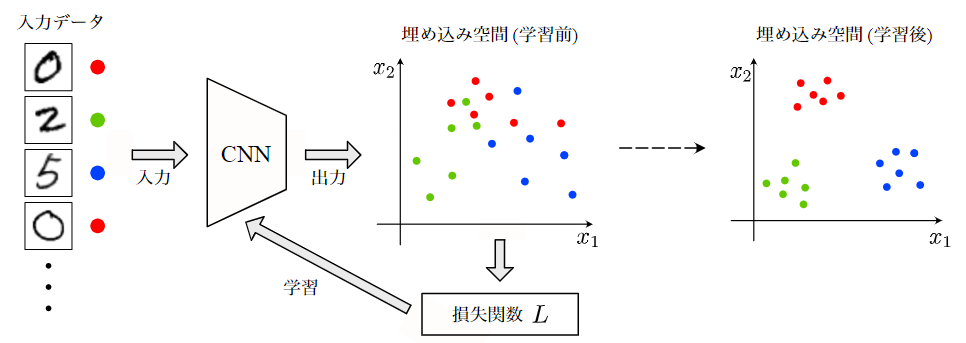
\includegraphics[width=13cm]{./capture/Metric_abstract.png}
  \caption{Metric Learningの概要}
  \label{fig:Metric_abstract}
\end{figure}
\par
例えば、画像認識においては、CNNのネットワーク構造自体を工夫しなくても、特徴空間を構成できるように学習を行うだけで、精度を向上させることができるようになるという利点がある。
\par
こうした特徴空間内のデータの配置を深層学習によって学習していくことを、深層距離学習と呼ぶ。深層距離学習は、Siamese NetworkやTriplet Networkといった手法が存在する。

\clearpage
\section{Siamese Network}
Siamese Network (シャムネットワーク) は、2つのデータを同時に入力し、それらのデータが同じクラスに属するかどうかを判定するネットワークである。入力$x_1, x_2$に対して出力$f(x_1), f(x_2)$であった場合、その特徴ベクトルの距離$D(f(x_1), f(x_2))$を計算し、損失関数$L$に入力することで、最適なネットワークのパラメータを学習する。
損失関数は、contrastive lossという名称があり、以下で表される。
\begin{align}
  L = \frac{1}{2} \left[ yD^2 + (1-y)\max(m-D, 0)^2 \right]
\end{align}
ここで、$y$は同じクラスに属するかどうかを示すラベルであり、$m$はマージンを示す。$D$は特徴ベクトルの距離であり、$D = ||f(x_1) - f(x_2)||$(ユークリッド距離)である。

この損失関数は、以下のように分解できる。
\begin{align}
  L &= yL_1 + (1-y)L_2\\
  L_1 &= \frac{1}{2}D^2\\
  L_2 &= \frac{1}{2}\max(m-D, 0)^2
\end{align}
$L_1$は、シンプルに距離の2乗であり、この損失関数を最適化することで、同じクラスに属するデータは近くに配置されるようになる(図\ref{fig:Siamese_L1})。一方で、$L_2$は、マージン$m$よりも離れたデータに対しては、損失が発生しないようになる。つまり、
\begin{align}
  \begin{cases}
    D < m & : L_2 = \frac{1}{2}(m-D)^2\\ 
    D \geq m & : L = 0
  \end{cases}
\end{align}
となる(図\ref{fig:Siamese_L2})。

\begin{figure}[htbp]
  \centering
  \begin{subfigure}[b]{0.45\textwidth}
    \centering
    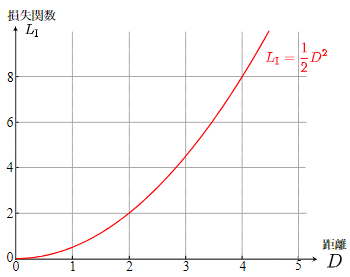
\includegraphics[width=\textwidth]{./capture/Siamese_L1.png}
    \caption{L1の損失関数}
    \label{fig:Siamese_L1}
  \end{subfigure}
  \hfill
  \begin{subfigure}[b]{0.45\textwidth}
    \centering
    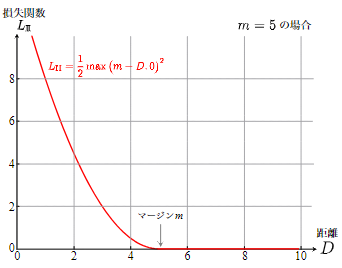
\includegraphics[width=\textwidth]{./capture/Siamese_L2.png}
    \caption{L2の損失関数}
    \label{fig:Siamese_L2}
  \end{subfigure}
  \caption{contrastive loss}
\end{figure}

深層距離学習では、類似データは近くに、異なるデータは遠くに配置されるように学習することで、特徴空間を構築する。そのため、Siamese Networkは、入力ペアが同じクラスの場合、$L_1$を、異なるクラスの場合、$L_2$を損失関数として用いることで、距離学習を行う。
\par
識別ラベル$y$は、同じクラスの場合は$y=1$、異なるクラスの場合は$y=0$となる。こうすることで、損失関数を一つの式でまとめて書いたものが、$L$(contrastive loss)である。
\par
この損失関数は大きな欠点が存在する。それは、異なるクラスのデータに対しては、$D=m$を超えた時点で最適化が終了するが、同じクラスのデータに対しては、$D=0$になるまで最適化し続けてしまうことである。この問題を解決するために、Triplet Networkが提案されている。

\clearpage
\section{Triplet Network}
Triplet Network (トリプレットネットワーク) は、Siamese Networkの欠点を解消するために提案されたネットワークである。Triplet Networkは、Anchor, Positive, Negativeの3つのデータを入力とし、AnchorとPositiveの距離を近づけ、AnchorとNegativeの距離を遠ざけるように学習する。
\par
Triplet Networkの損失関数は、triplet lossと呼ばれ、以下で表される。
\begin{align}
  L = \max(D_p- D_n + m, 0)
\end{align}
ここで、$D_p$はAnchorとPositiveの距離、$D_n$はAnchorとNegativeの距離、$m$はマージンを示す。
\par
triplet lossは、以下のように場合分けできる。
\begin{align}
  \begin{cases}
    D_p + m > D_n & : L = D_p - D_n + m\\
    D_p + m \leq D_n & : L = 0
  \end{cases}
\end{align}
$D_p+m > D_n$という状況は、NegativeとAnchorの距離$D_n$がPositiveとAnchorの距離$D_p$から、マージン$m$分大きな領域内に入っていて、十分に類似しないサンプルの位置を話すことができていない状況を示している。逆に、$D_p+m \leq D_n$という状況は、NegativeとAnchorの距離$D_n$がPositiveとAnchorの距離$D_p$から、マージン$m$分大きな領域の外にあるため、十分に異なるサンプル同士が離れた状況になる。
\par
Triplet Networkは、コンテキスト情報をアンカーに与えることで、Siamese Networkではできなかった、複数のクラスに対する距離学習を行うことができる。例えば、
\begin{itemize}
  \item 画像A : 男性, 鈴木
  \item 画像B : 男性, 田中
\end{itemize}
というデータが与えられた場合、どういったタスクを行うかによって、AとBの距離を近づけるか、遠ざけるかが変わる。Triplet Networkは、Anchorに画像C: 女性, 鈴木を与えることで、AとCの距離を近づけ、BとCの距離を遠ざけるように学習するし、Anchorに画像D: 男性, 田中を与えることで、AとDの距離を遠ざけ、BとDの距離を近づけるように学習する。
\par
ただし、Triplet Networkも、問題点がいくつか存在する。例えば、学習が停滞しやすい、クラス内距離がクラス間距離より小さくなることを保証しない、といった問題がある。これらの問題を解決するために、Quadrupt lossと呼ばれる損失関数が提案されている。

\section{MAML(メタ学習)}
MAML(Model-Agnostic Meta-Learning)は、少ないデータによる学習を行うための手法である。MAMLは、メタ学習と呼ばれる手法の一つであり、メタ学習は、学習の学習を行う手法である。
\par
深層学習モデル開発に必要なデータ量は膨大であり、特に画像認識などのタスクにおいては、数十万枚の画像データが必要とされる。例えば、MNISTは手書き数字のデータセットであり、7万枚の画像データが用意されている。また、ImageNetなら約120万枚, Open Image Dataset V6は、約900万枚の画像データが用意されている。これらのデータに対して、ラベル付けを行うためには、人手でラベル付けを行う必要があり、膨大な時間とコストがかかる。
\par
こうした問題から、少ないデータで如何にして学習を行うかが重要となる。
\par
少ないデータで学習を行う手法として、事前学習、転移学習、ファインチューニングという一連の手法は比較的古くから存在している。この手法は、大規模なデータセットで学習したモデルを、新しいタスクに適用することで、少ないデータで学習を行うことができる一方で、必ずしも最適な重みを得ることができるとは限らないという問題があった。
\par
MAMLは、この問題を解決するために提案された手法であり、様々なタスクに合わせて、ファインチューニングを行うことで、あらゆるタスクに対して有効な汎用的なモデルを学習することができる。
\par
MAMLは、以下のような手法で学習を行う。
\begin{enumerate}
  \item タスク集合$\tau$から、タスク$\tau_i$をランダムに選択する (Inner Loop)
  \item タスク$\tau_i$に重み$\theta$を最適化し、新しい重み$\theta'_i$を得る (Inner Loop)
  \item すべてのタスクに対して重みを更新し、重みの集合$\Theta=(\theta'_1, \theta'_2, \cdots)$を得る (Outer Loop)
  \item 集めた重みで共通重み$\theta$を更新する (Outer Loop)
  \item 1-4を繰り返す
\end{enumerate}
この手法により、少ないデータで効果的に学習を行うことができる。
しかし、MAMLは、計算コストが高いという問題がある。この問題を解決するために、First-order MAML(2次以上の勾配を無視), Reptile(InnerLoopの逆伝播を行わない)という手法が提案されている。

\clearpage
\section{グラフ畳み込み (GCN)}
グラフ畳み込み (Graph Convolutional Network, GCN) は、グラフデータに対して畳み込み演算を行うニューラルネットワークである。グラフデータは、ノードとエッジから構成されるデータであり、例えば、ソーシャルネットワーク、化合物の構造、交通ネットワーク、新型コロナの感染経路などが挙げられる。
\par
グラフ畳み込みでは、まず対象のノードに対して、その近傍のノードとの情報を集約する演算を行う。その後、次に近いノードとの情報を集約する演算を行い、これを繰り返すことで、グラフ全体の情報を集約する。
\par
グラフ畳み込みの手法には、Spatial GCN, Spectral GCN, ChebNet, GraphSAGE, GAT, GraphWavelet, Graph Isomorphism Network (GIN) などが存在する。これらの手法は、グラフデータの特性に合わせて、畳み込み演算を行う手法が異なる。

\clearpage
\section{Spatial GCN}
Spatial GCNは、グラフデータに対して、クラスタリングを繰り返し、空間的な畳み込み演算を行う手法である。Spatial GCNは、グラフデータの隣接行列を用いて、ノードの特徴量を更新する。
Spatial GCNは規則性が弱いものであっても、規則性を見出すことができるかもしれないという強みがある。一方で、次元が低く近傍のある場所が限られる場合、広い範囲で重みを持たせにくいという弱点がある。

\clearpage
\section{Spectral GCN}
Spectral GCNは、グラフデータに対して、フーリエ変換を用いて畳み込み演算を行う手法である。Spectral GCNは、グラフデータのラプラシアン行列を用いて、ノードの特徴量を更新する。
Spectral GCNは、グラフデータの特性を捉えることができるが、グラフデータのラプラシアン行列の固有値分解を行うため、計算コストが高いという問題がある。また、グラフ間でサイズや構造が変わるとパラメータの使いまわしができないという問題もある。


\clearpage
\paragraph{参考文献}
\begin{enumerate}
  \item 岡谷貴之/深層学習 改訂第2版 [機械学習プロフェッショナルシリーズ]/ 講談社サイエンティフィク/ 2022-01-17
\end{enumerate}

\newpage
\end{document}